\section{Random Forest} %4.5

To use Random Forest, three parameters had to be determined which are the number of total features, the number of trees, and the number of features that randomly applied in each tree (\sys{mtry}). 

Firstly, nine out of eleven features were applied on this algorithm based on correlation matrix. Then, the "tree number vs out-of-bag error" graph (the right of Figure \ref{4.2.6-RF-200Trees-5Features}) was plotted. Based on different \sys{mtry} values, when the tree number approaches 200, the out-of-bag error tends to be stable. Hence, 200 was chosen as the tree number of this model.


\begin{figure}[htbp]
\center
  \begin{subfigure}{7.5cm}
    \centering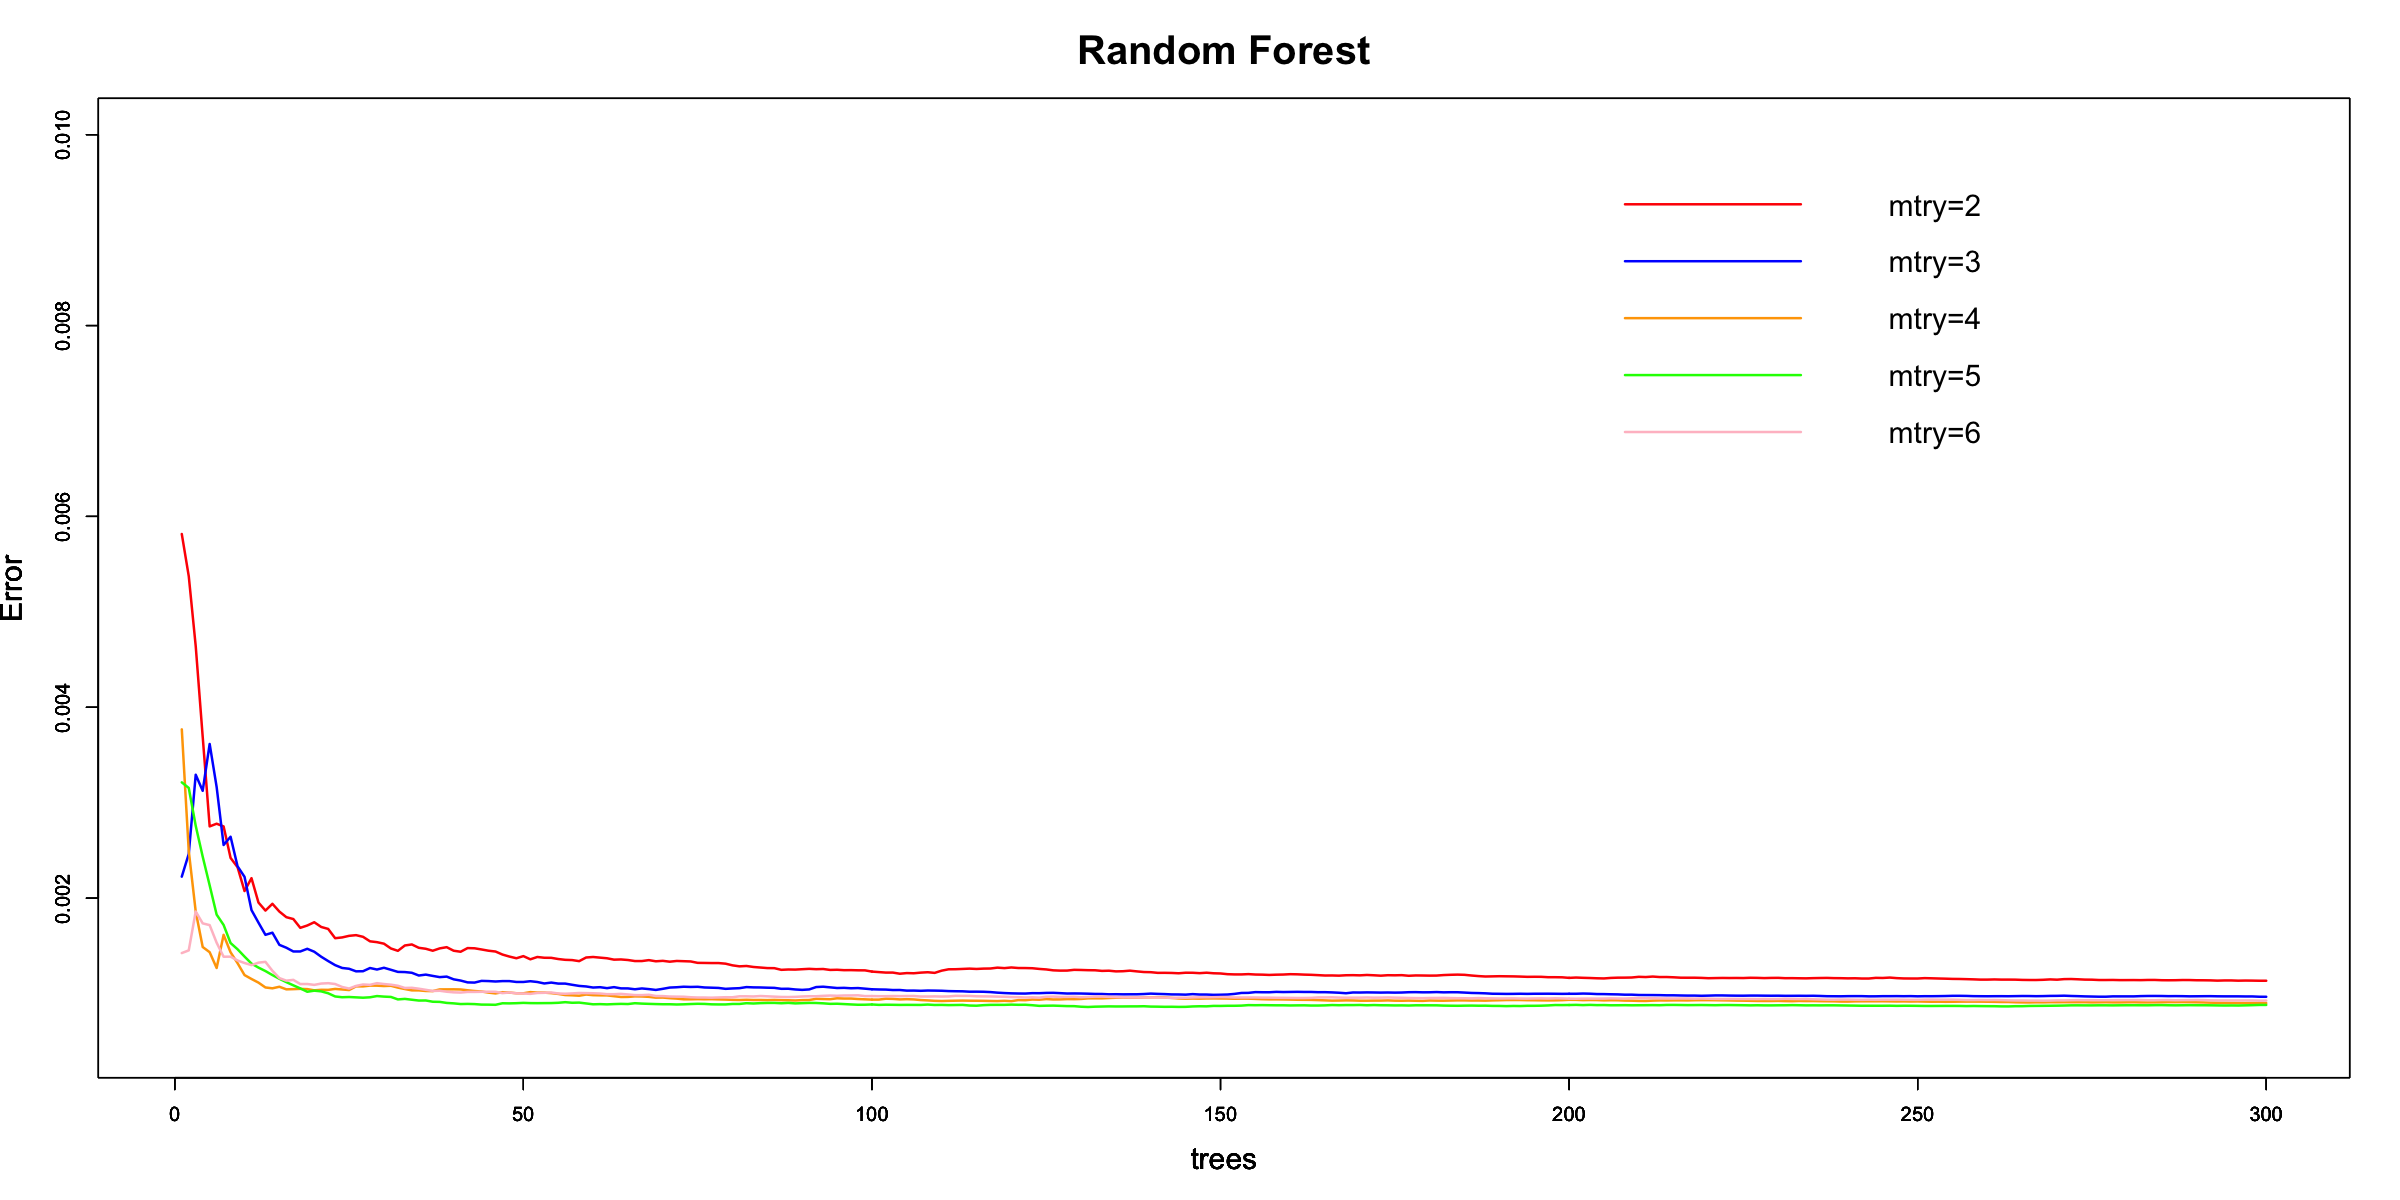
\includegraphics[width=7cm]{Figure/4.2.4-RF-200TreesStable.png}
  \end{subfigure}
  \begin{subfigure}{7.5cm}
    \centering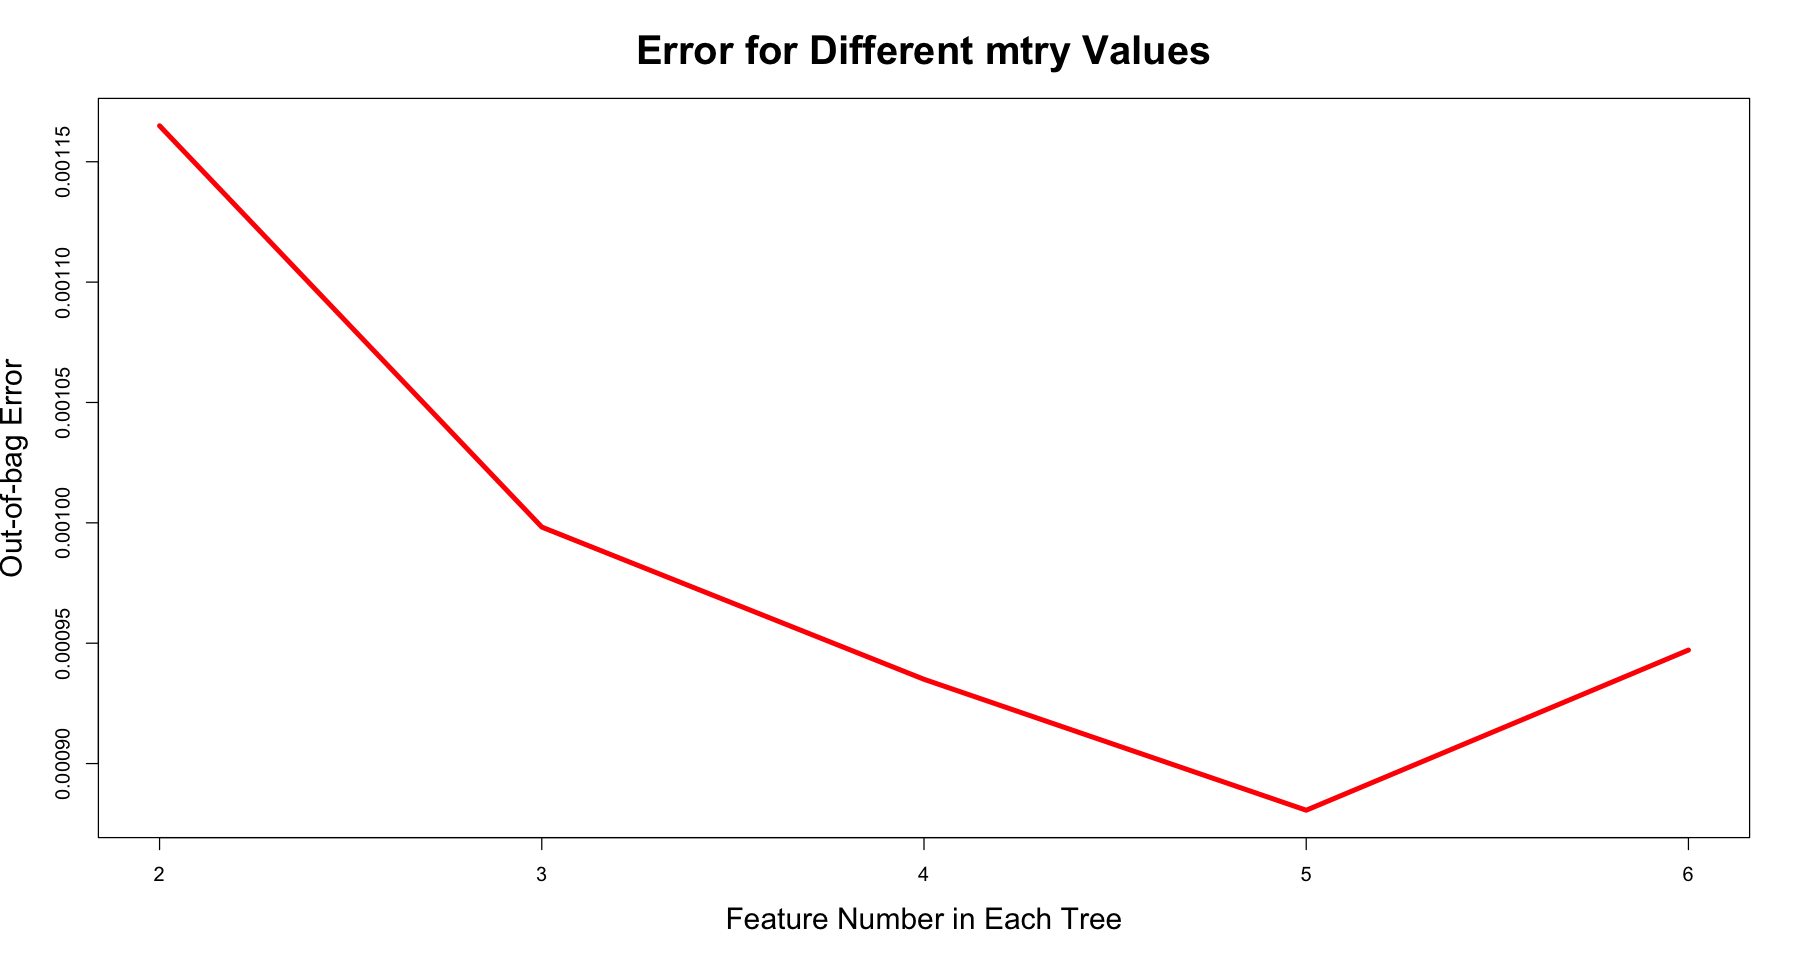
\includegraphics[width=7cm]{Figure/4.2.4-RF-5Features.png}
  \end{subfigure}
  \caption{Left: Check the error stability of random forest with different number of trees. Right: Check the out-of-bag error of random forest with different number of features in each tree when three number is 200.}
  \label{4.2.6-RF-200Trees-5Features}
\end{figure}

Moreover, the choice of the \sys{mtry} value is also important. Based on the selected tree number, different out-of-bag errors would be obtained by using different \sys{mtry} values. Through comparison, feature number in each tree was selected as 5 which corresponds with the minimum out-of-bag error.

After parameter was selected, Random Forest model was trained and tested. The MSE value is 0.00105 which is much smaller than the previous models. Observing the fitting diagram (bottom of Figure \ref{4.2.6-RFMSE}), it was found that dots were distributed in a narrow area fitting the straight line $y=x$, which indicates a robust fitting performance.

\begin{figure}[htbp]
\centering
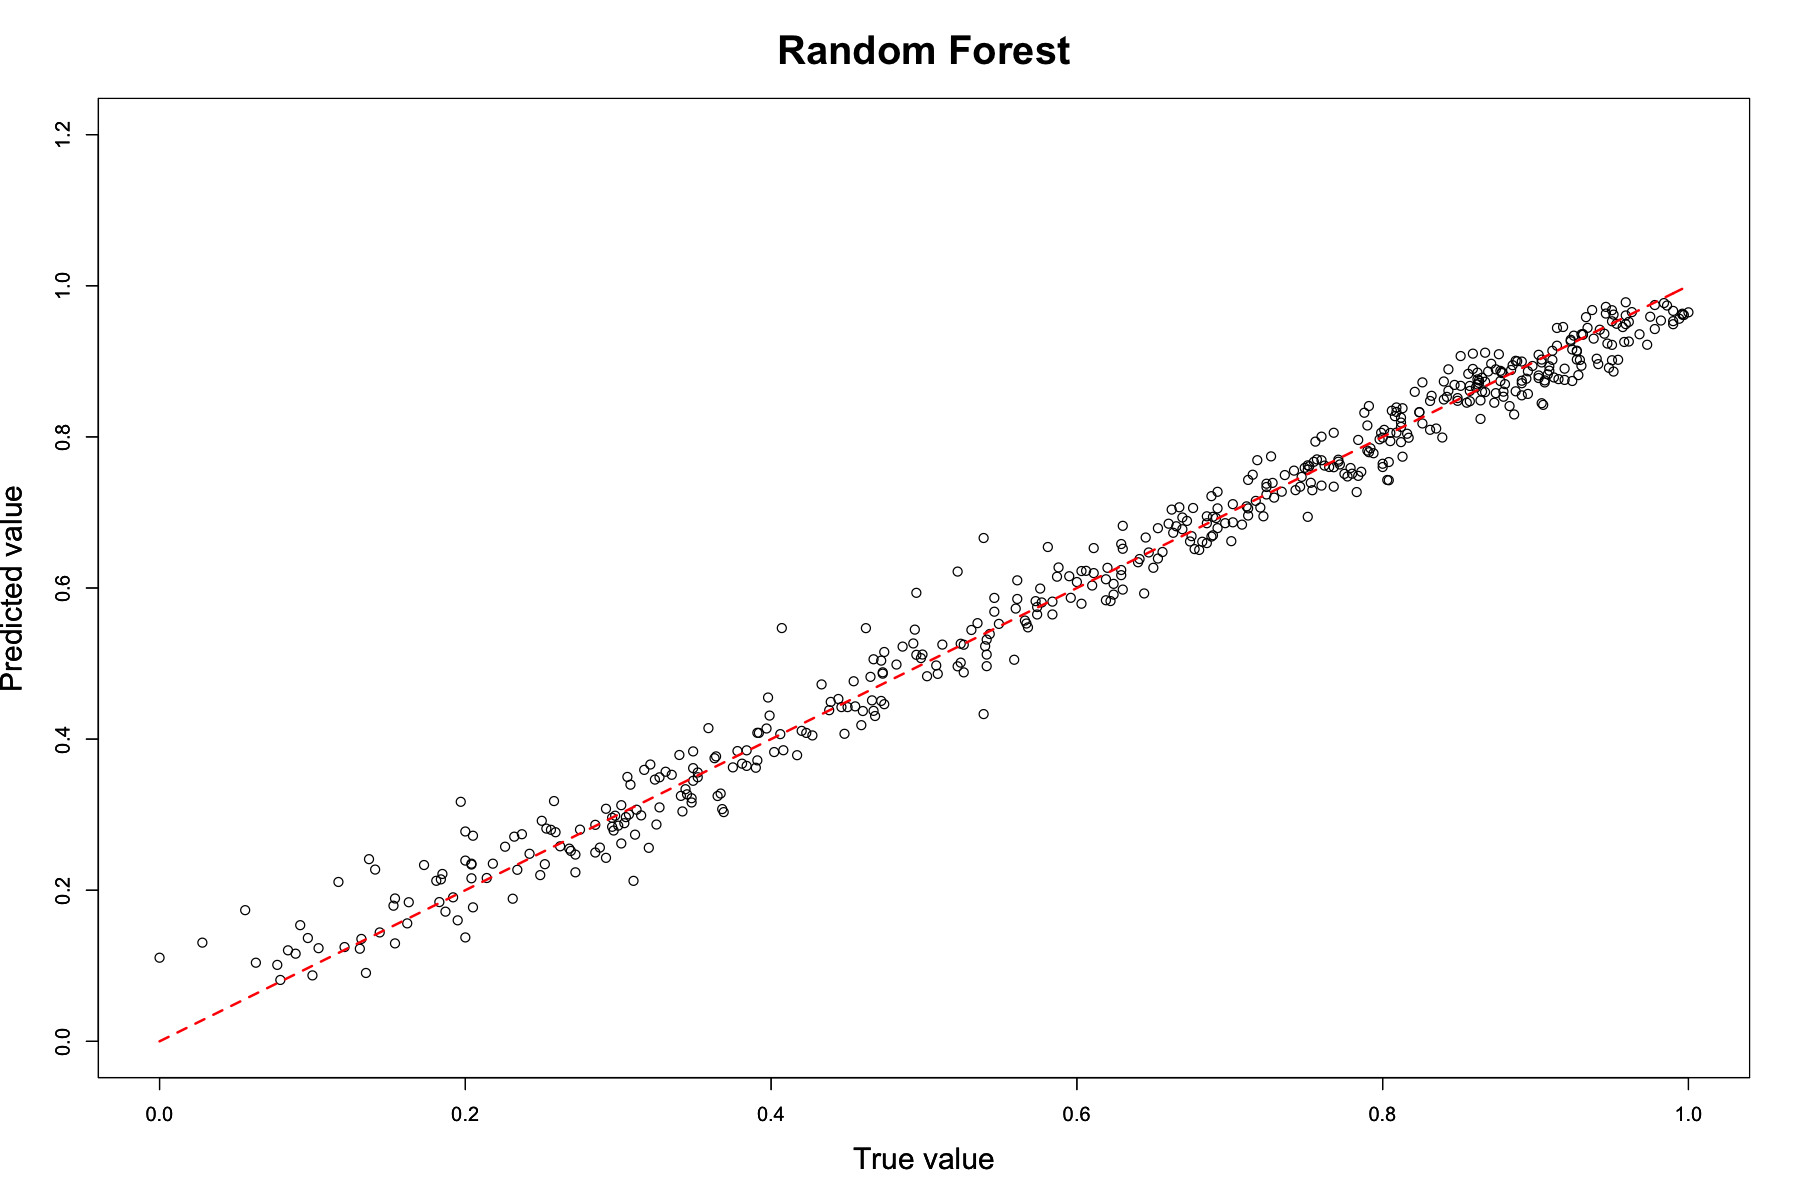
\includegraphics[width = 1.0\textwidth]{Figure/4.2.4-RF.png}
\caption{The predicted Arctic sea ice extent value vs the real Arctic sea ice extent value with \textbf{Random Forest} (200 trees, 5 features). The red referenced dotted line represents the straight line y=x. Mean Square Error (MSE) is \textbf{0.00105}.}
\label{4.2.6-RFMSE}
\end{figure}



\newpage